\documentclass[12pt]{article}
\usepackage{amsmath, amssymb}
\DeclareMathOperator{\Tr}{Tr}
\usepackage{bbold}
\usepackage{graphicx}
\usepackage[pdfencoding=auto, psdextra]{hyperref}
%To deal with an error "Package hyperref Warning: Token not allowed in a PDF string"
\pdfstringdefDisableCommands{\def\varepsilon{\textepsilon}} 
\graphicspath{{images/}}
\usepackage[top = 2.5cm, bottom = 2.5cm, left = 2.5cm, right = 2.5cm]{geometry}
\usepackage{natbib} % To cite
\usepackage[ruled,vlined]{algorithm2e}

\renewcommand{\thesection}{S\arabic{section}}
\renewcommand{\theequation}{S\arabic{equation}}
\renewcommand{\thetable}{S\arabic{table}}
\renewcommand{\thefigure}{S\arabic{figure}}

\title{Supplementary Material for:\\The role of competition versus cooperation in microbial community coalescence}
\author{Pablo Lechón, Tom Clegg, Jacob Cook, Thomas P. Smith, Samraat Pawar}

% Everywhere there's a direct reference to a main text equation I have put a comment saying "check equation number before submission"
% Before submission should crt+f that phrase and check equal equation

\begin{document}
\maketitle

\tableofcontents

\newpage

\section{Relationship with other microbial consumer-resource models}

Here we describe how our model is related to two other recent ones that have been used to study microbial community assembly and coalescence. The mapping between the notation used in \cite{Tikhonov2016} (T), \cite{Marsland2019} (M) and those used here is provided in the following table:\\
\begin{center}
    \begin{tabular}{ |l|c|c|c| } 
		\hline
		Notation for... & M & Here & T \\ 
		\hline
		Species index & $ i $ & $ {\alpha} $ & $\vec{\sigma}$ \\ 
		Species abundance & $ N_i $ & $ n_{\alpha} $ & $ n_{\sigma} $ \\ 
		Resource a species can harvest & $ \vec{c_{i}} $ & $ \vec{c_{{\alpha}}} $ & $ \sigma_i $ \\ 
		Resource supply & $ \kappa_{\alpha}$ & $ \kappa_j $ & $ R_i $ \\ 
		Dilution rate & $ \tau_{\alpha} $ & $ \infty $ & $ NA $\\
		Minimal resource requirement & $ m_i $ & $ z_{\alpha} $ & $ \chi_{\vec{\sigma}} $ \\ 
		Resource weight & $ w_{\alpha} $ & $ \vec{1} $ & $\vec{1}$ \\ 
		Resource $ \rightarrow $ biomass conversion factor & $ g_i $ & $ g_{\alpha} $ & $ (\tau_0\chi_{\vec{\sigma}})^{-1} $ \\ 
		Leakage factor & $ l_{\alpha} $ & $ l $ & 0 \\
		Metabolic matrix & $ D_{\alpha\beta} $ & $ (D_{kj})^T $ & NA \\ 
		\hline
    \end{tabular}
\end{center}

\subsection*{With \cite{Marsland2019}'s Model}

Our model differs from the version used in \cite{Marsland2019} in the following respects:
(i) all resources contain the same amount of energy (taken to be 1 for simplicity), (ii) a type I functional response, (iii) binary consumer preferences, (iv) a shared core metabolism encoded in $D$, (v) a common leakage fractions for all species and resources, and (vi) a complex environment where all resources are externally supplied in equal amounts. We address the implications of these assumptions in the Discussion section.  
\begin{enumerate}
    \item All resources contain the same amount of energy ($\omega_j = 1$).
    \item We only consider a type-1 functional response ($c(R_j) = R_j$).
    \item Consumer preferences are binary, instead continuously distributed between 0 and 1.
    \item Dilution rate is very high, such that $\tau^{-1}\approx 0$
\end{enumerate}

\subsection*{With \cite{Tikhonov2016}'s Model}

 \cite{Tikhonov2016} did not explicitly model resource dynamics, but we can establish the relationship between that model and the one used here, as follows. Our consumer-resource model is,
\begin{align}
    \begin{split}
        \frac{dn_{\alpha}}{dt} &= g_{\alpha}n_{\alpha}\left((1-l)\sum_j c_{\alpha j}R_j - z_{\alpha}\right)\\
        \frac{dR_{j}}{dt} &= \kappa_j - \sum_{\alpha}n_{\alpha}c_{\alpha j}R_j + l\sum_{\alpha k}n_{\alpha}D_{kj}c_{\alpha k}R_k.
    \end{split}
    \label{eq:model}
\end{align}
In the limit when there is no leakage ($l = 0$), we can make the assumption that molecular (resource) dynamics are faster than population dynamics, and therefore that resource concentration $R_j$ at any moment quickly equilibrates to reflect the instantaneous demand, i.e., $ dR/dt \approx 0 $. This allows us to separate the time scales between resource and population dynamics, recovering the model used by \cite{Tikhonov2016}:

\begin{equation*}
    \begin{aligned}
		\frac{dn_{\alpha}}{dt} &= g_{\alpha}N_{\alpha}\Big(\underbrace{\sum_j c_{{\alpha}j}\frac{\kappa_j}{\sum_{\alpha}N_{\alpha}c_{{\alpha}j}} - z_{\alpha}}_{\text{Resource surplus }\Delta_{\alpha}}\Big)\\
		R_j &= \frac{\kappa_j}{\sum_{\alpha}N_{\alpha}c_{{\alpha}j}}\\
    \end{aligned}
\end{equation*} 

\section{Cost function}\label{cost_function}
    
The cost function used in our model (Eq \ref{eq:model}) ensures that neither specialists or generalists are systematically favoured during community assembly, and corresponds to the assumption of approximate neutrality \citep{Tikhonov2016, Tikhonov2017, Tikhonov2018}.
Species $\alpha$ will increment its abundance when its surplus term in Eq \ref{eq:model} is greater than 0;
\begin{equation}\label{eq:cost_harvest}
    \frac{1}{g_{\alpha}n_{\alpha}}\frac{dn_{\alpha}}{dt} = (1-l)\sum_j c_{\alpha j}R_j - z_{\alpha} > 0
\end{equation}
That is, species able to maintain positive growth for the lowest concentration of resources will be favoured. This can be achieved by either reducing the cost $z_{\alpha}$ or increasing the number of resource preferences in Eq \ref{eq:cost_harvest}. However, if one imposes the constraint $z_{\alpha} = \sum_j c_{\alpha j}$, the condition to maintain positive growth becomes 
\begin{equation*}
    R_j - \chi_0 > 0
\end{equation*}
% check equation number before submission
Which is independent of the number of preferences of the consumer; that is, species are neutral under this assumption. To break this degeneracy, and place our model in the regime of approximate neutrality, we introduce a small random fluctuation term, $\epsilon$ in Eq 2 of the main text. 

\section{Competition and Facilitation Metrics}

In the model system (Eq \ref{eq:model}), competition for resources exists because the metabolic preferences vectors of all species in the community will generally overlap. We define intrinsic competition between a pair of species $(\alpha, \beta)$ as the level of overlap between their metabolic preferences, independent of their environment's state. We calculate this metabolic overlap by counting the number of common preferences. Since these are binary, taking the scalar product of the two preference vectors yields the number of common elements between them,
\begin{equation*}
    (C_i)_{\alpha \beta} = \sum_kc_{\alpha k}c_{\beta k}.
\end{equation*}
This intrinsic competition becomes effective competition when we consider the environmental states experienced by the consumers, which change due to biotic and abiotic factors.

The resources available in the environment can either be externally supplied through $\kappa$ or leaked by consumers through $l$ and $D$. Depending on their origin, effective competition for resources is calculated differently. Consider the resource abundance landscape of a system as its dynamics unfold. Initially ($t = 0$) species are inoculated in an environment where all resources are externally supplied. As the dynamics play out, a fraction $l$ of the externally supplied resource abundance vector is mapped into another vector of abundances through leakage according to the core metabolism $D$. When the system reaches equilibrium, both resource abundance profiles (the externally supplied and the one leaked by consumers) coexist, so effective competition (henceforth, just `competition') needs to be calculated differently for each resource profile. We calculate the competition  between a given pair of species on abiotically vs biotically generated resources as follows.

The competition for each abiotically-generated resource is weighted by the normalized resource supply 
$$\tilde{\kappa} = \vec{\kappa}/\text{max}(\vec{\kappa}),$$
with the interaction strength given by the non-leaked fraction $1 - l$ (fraction of any resource that is effectively consumed abiotically ). Thus, the overall competition $C_a$ between the species pair $(\alpha, \beta)$ for abiotically-generated resources  must be
\begin{equation}\label{eq:abiotic}
	(C_a)_{\alpha\beta} = (1-l) \sum_k \tilde{\kappa}_kc_{\alpha k}c_{\beta k}.
\end{equation}

Now consider the competition between species $\alpha$ and $\beta$ for biotically-generated resources (which have been leaked to the environment), $C_b$. There will only be competition for the $k^{th}$ biotically-generated resource when both the following two conditions hold: 1) $\alpha$ or $\beta$ consume resource $j$ and leak a fraction of it in the form of resource $k$; 2) $\alpha$ and $\beta$ both consume $k$. Mathematically, this combination of conditions implies:
\begin{equation}\label{eq:little_biotic_term}
    (C_b)^{k\rightarrow j}_{\alpha \beta} \propto D_{jk}\left(c_{\alpha j} + c_{\beta j}\right)c_{\alpha k}c_{\beta k}.
\end{equation}

In the case of abiotic competition, it was straightforward to see that the interaction strength of abiotic competition is the consumption fraction $1-l$. Intuitively, one would think that $l$ is the interaction strength for competition on biotically-generated. Formally, we can perform think of the harvest-leaking process as a infinite discrete succession of consumption and leakage cycles. When a species harvests resource $j$ from the environment, it intakes a fraction $1-l$ and leaks back a fraction $l$ in the form of other resources (first two arrows in Fig  \ref{fig:cycling_scheme}). The leaked resources become part of the available resource pool, and are competed for in a second cycle of consumption, with intake fraction $l(1-l)$. This process extends up to $n$ cycles, (with $n \rightarrow \infty$),  as illustrated in Fig \ref{fig:cycling_scheme}, so that at cycle $n$, the fraction of harvested resource is $l^n(1-l)$. The strength of the biotic competition and facilitation links, $B$, is calculated by summing the fraction of ingested resource over all cycles as
\begin{equation*}
    B = \sum_{n = 1}^{\infty}\ l^n(1-l)= (1-l)\left(\sum_{n = 0}^\infty l^n -1\right) = (1-l)\left(\frac{1}{1-l} - 1\right) = l.
\end{equation*}
As expected, the strength factor for biotic links is $l$, the fraction of resources originally leaked. Note that this result depends on the convergence of the geometric series, which is only true when $l < 1$. In the trivial case $l = 1$, then $B = 0$, and the system would have neither competitive nor facilitative interactions.

\begin{figure}[t]
	\centering
	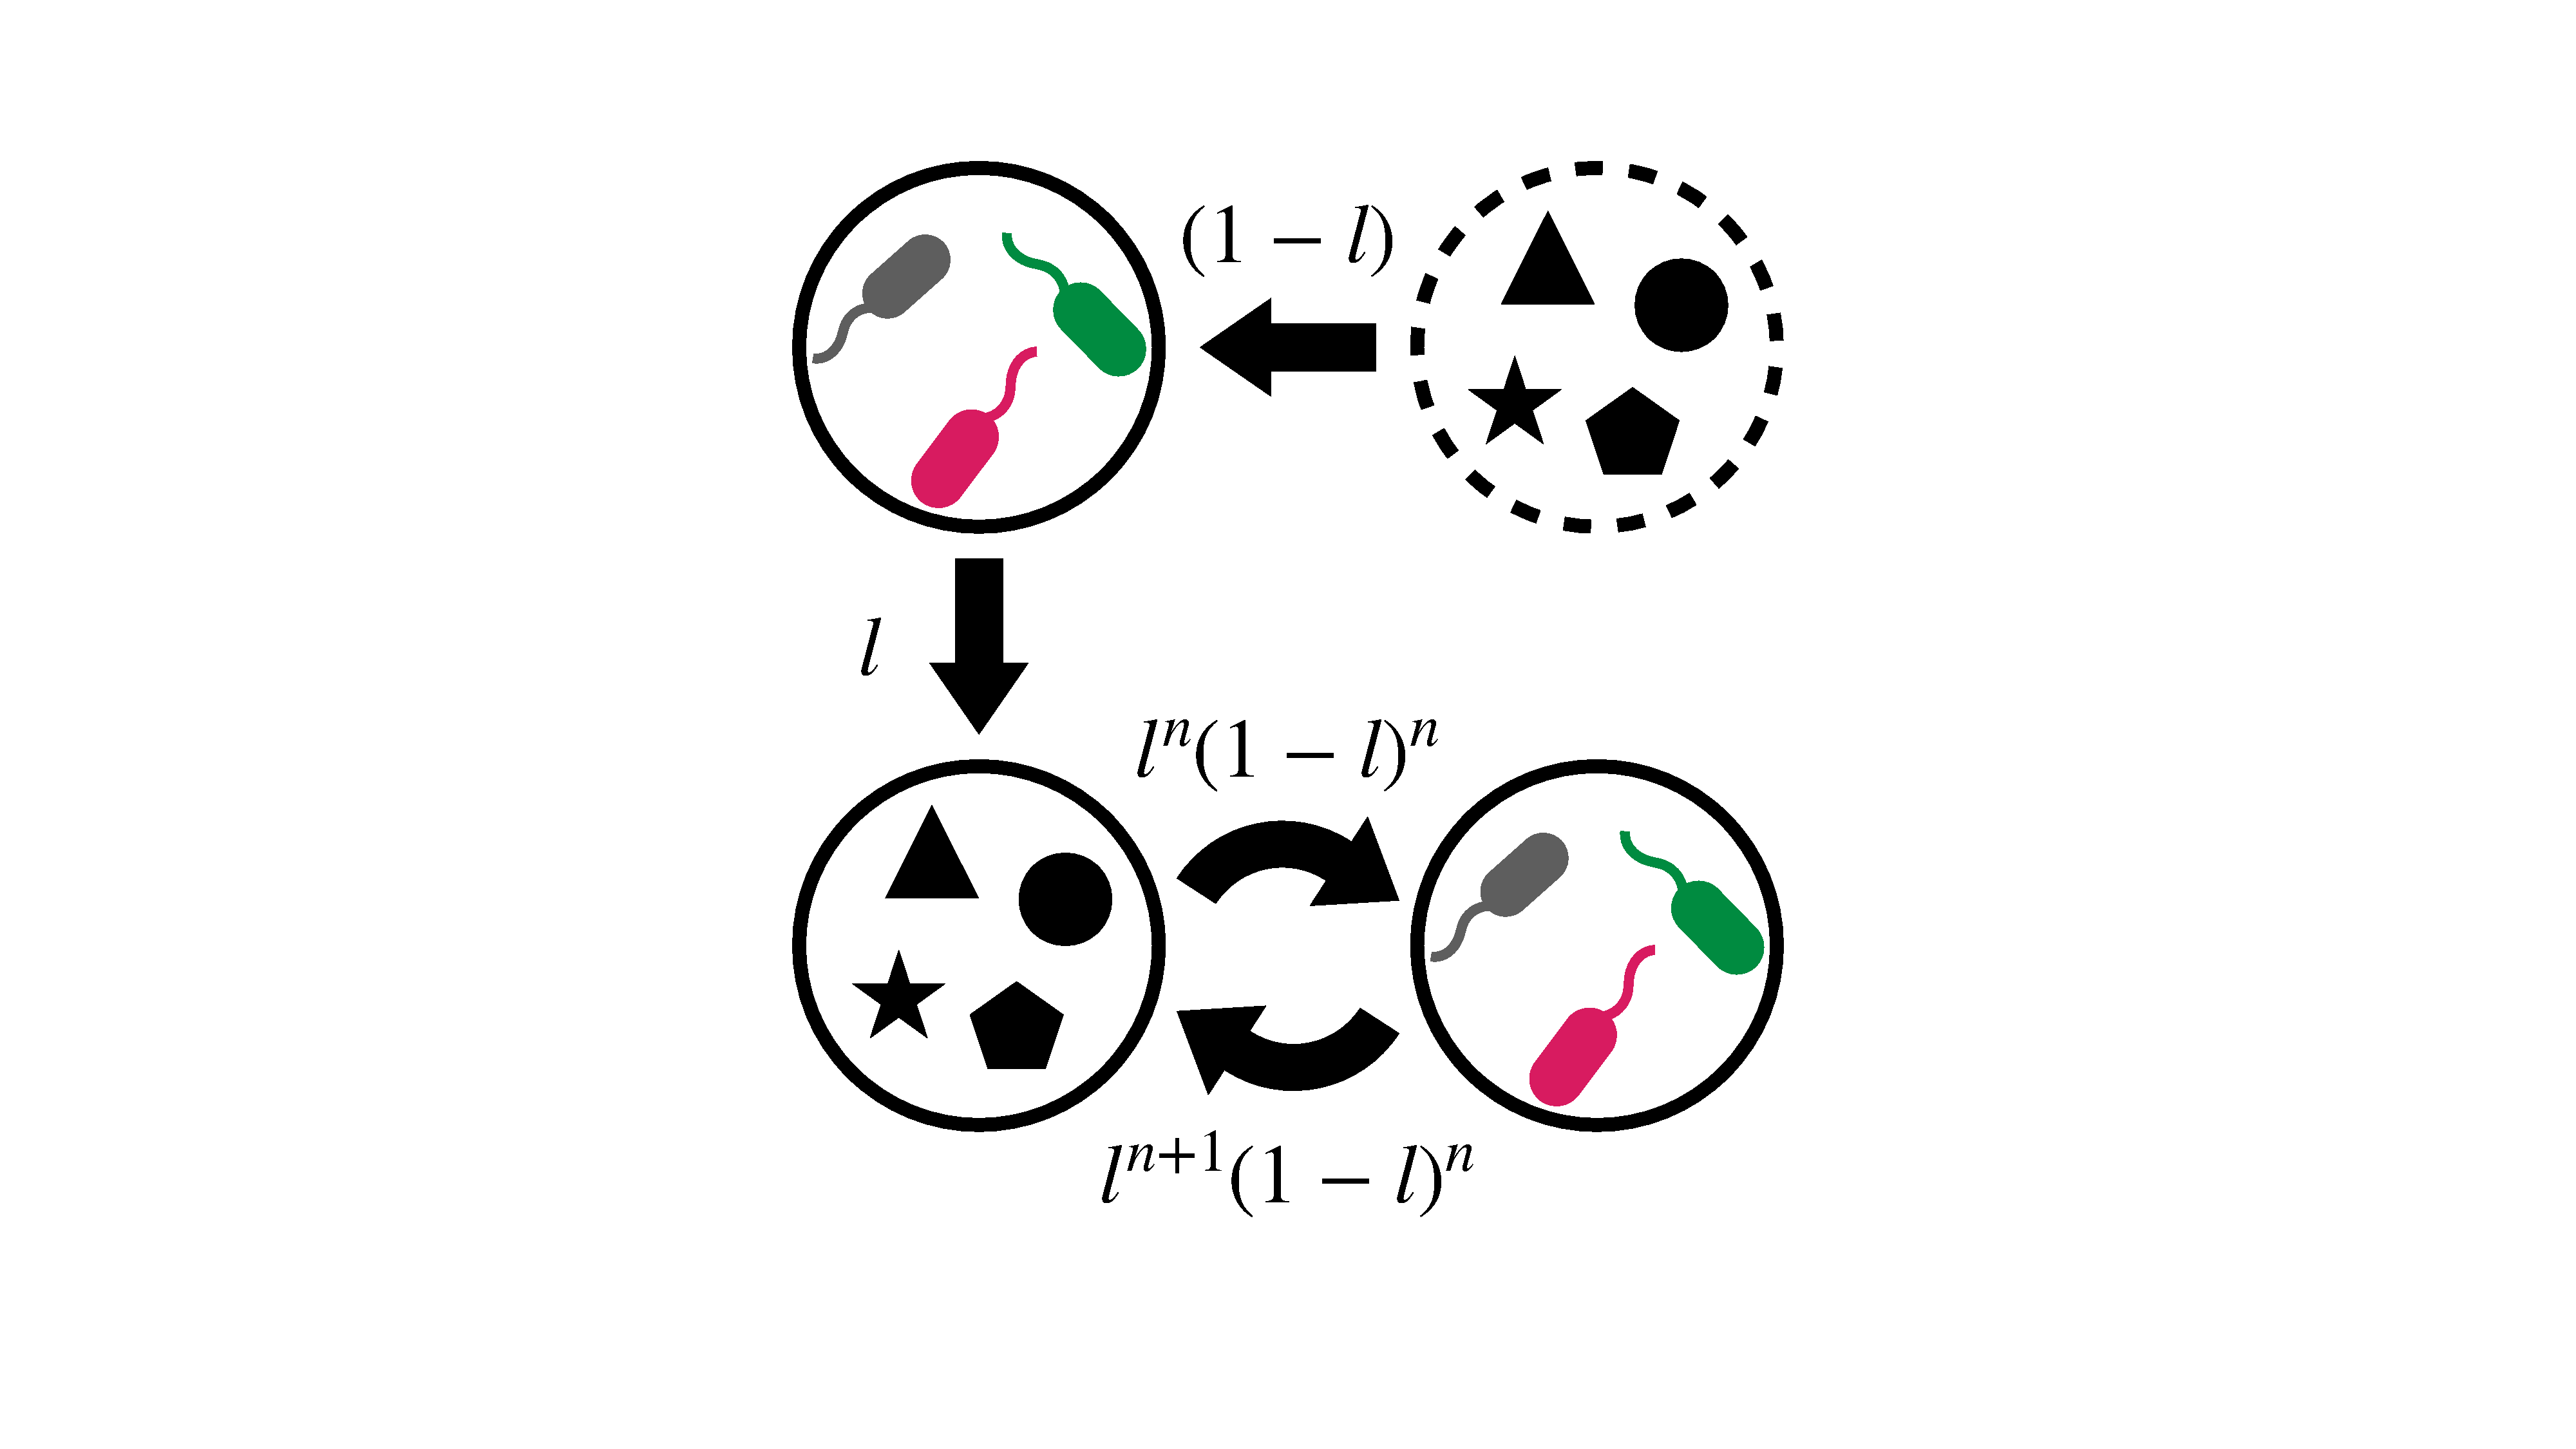
\includegraphics[width=0.4\textwidth]{cycling_scheme.pdf}
	\caption{\textbf{Mechanism of resource recycling}. The species in this model consume the resources that come through the supply rate $\kappa$ (abiotic uptake, top arrow) and leak a fraction $l$ back to the environment (left arrow). The leaked resources can be harvested again by the species in the community (biotic uptake, bottom arrows). This can be modeled as an infinite series of consecutive cycles of uptake and leakage where the amount of resources consumed by each strain decreases by a factor of $l$, after each cycle.}
	\label{fig:cycling_scheme}
\end{figure}

Then, the total competition between the species pair $(\alpha, \beta)$ for biotically-generated resources is the sum of the terms that arise from expression \ref{eq:little_biotic_term} when spanning the full resource set, weighted by $l$:
\begin{equation}\label{eq:biotic}
	(C_b)_{\alpha\beta} = l \sum_{jk} \tilde{\kappa}_jD_{jk}\left(c_{\alpha j} + c_{\beta j}\right)c_{\alpha k}c_{\beta k}.
\end{equation}
Note that the factor $\tilde{\kappa}_j$ is necessary in both measures of competition (equations \ref{eq:abiotic} and \ref{eq:biotic}) because all  resources are externally-supplied when they first enter the system, and so we need to account for possible differences in the external resource supply rate. 

The two types of competition presented here, are merely a formal classification, since consumers cannot tell apart biotically and abiotically-generated resources. Therefore, the total competition between species pair $(\alpha, \beta)$ is the sum of the two terms
\begin{equation}\label{eq:competition}
    (C_T)_{\alpha \beta} = (C_a)_{\alpha \beta} + (C_b)_{\alpha \beta}.
\end{equation}

Next, we consider facilitation. Facilitation links form when a species leaks resources (metabolic by-products) that are used by another species. Therefore, the facilitation of species $\alpha$ towards species $\beta$ when the former consumes resource $j$ and releases $k$ will be non-zero when 1) species $\alpha$ produces $k$ as a metabolic by-product when consuming $j$, and 2) species $\beta$ consumes $k$. Analogous to the case of competition for biotically-generated resources (Eq~\ref{eq:biotic}), the strength of these interactions is also given by $l$ and the factor $\tilde{\kappa}_j$. Combining these conditions, the total facilitation of species $\alpha\rightarrow \beta$ will be
\begin{equation}\label{eq:facilitation}
    F_{\alpha \beta} = l\sum_{jk} \tilde{\kappa}_jc_{\alpha j}D_{jk}c_{\beta k}.
\end{equation}
Note that facilitation is directional, which implies that the community facilitation matrix $F_{\alpha \beta}$ is not symmetric. On the other hand, the community competition matrix $(C_T)_{\alpha \beta}$ is symmetric, since competition is not directional.  

Averaging the matrices of pairwise metrics \ref{eq:competition} and \ref{eq:facilitation} yields a proxy of the community-level competition and facilitation. The matrix diagonals are left out of this averaging because we are only interested in inter-specific competition and facilitation. Additionally, we only consider the upper diagonal elements of the symmetric competition matrix. Then, the community-level competition and facilitation measures are given by
\begin{equation*}
    \mathcal{C} =  \langle C_{T_{\alpha \beta}} \rangle_{\alpha \neq \beta}~~\&~~\mathcal{F} =  \langle F_{\alpha \beta} \rangle_{\alpha \neq \beta},
\end{equation*}
respectively.

\section{Modulating cohesion levels}\label{derivation_micro_structure_supp}

We are interested in generating communities spanning a broad range of cohesion levels, i.e., different competition and facilitation levels. These can be modified by sampling $ c_{{\alpha}j} $ and $ D_{jk} $ respectively with certain constraints.

\subsection*{Modulating competition level}
First, let us consider the problem of modulating the competition level of the community by sampling the metabolic preferences for each strain, encoded in  $ c_{{\alpha}j} $. Each species $ {\alpha} $ has a binary vector $ \vec{c_{\alpha}} $ of length $ m $ that specifies if resource $ j $ is used ($ c_{{\alpha}j} = 1 $) or not ($ c_{{\alpha}j} = 0 $). \\
The metabolic preference matrix $ C $ is constructed by sampling its rows $ \vec{c_{\alpha}} $ sequentially. The process of sampling $ \vec{c_{\alpha}} $ is two-fold. We first sample $ m_{\alpha} $, the number of resources that species $ {\alpha} $ uses, from an exponential distribution. This choice is supported by experimental evidence \citep{Sung2017}. Second, to determine which resources are used by species $ {\alpha} $, we sample $ m_{\alpha} $ resources with probability vector $ \vec{p_{\alpha}} $. Note that in this sampling scheme, `iteration number' and `species' are equivalent, and denoted by index ${\alpha}$.\\
For species $ {\alpha} = 1 $ all resources have the same probability of being sampled $ 1/m $, where $ m $ is the total number of resources. This assumption is consequent with the absence of a resource hierarchy, since they all carry the same energy. After each iteration, the sampling probability of each resource changes according to what has been sampled previously. Let $ d_{{\alpha}j} $, denote the cumulative demand of resource $ j $ when the metabolic preferences of species $ {\alpha} $ are sampled. That is, the number of consumers of resource $ j $ at iteration $ {\alpha} $.
\begin{equation*}
	d_{{\alpha}j}  = \sum_{i = 1}^{{\alpha}}c_{ij}.
\end{equation*}
Based on $ d_{{\alpha}j} $, I then compute the probability that species $ {\alpha} $ is assigned resource $ j $ as one of its preferences
\begin{equation}\label{eq:sampling_probability_supp}
	p_{{\alpha}j}= (1-k_c) \frac{1}{m}  + k_c \frac{d_{{\alpha} -1j}}{\sum_{j}d_{{\alpha}-1j}},
\end{equation}
where the denominator represents the total number of preferences sampled up until iteration $ {\alpha}-1 $, and acts as a normalization constant, and together with the numerator represents the normalized cumulative demand (Eq~7 main text),
\begin{equation}
    \tilde{d}_{\alpha  -1j} = \frac{d_{{\alpha} -1j}}{\sum_{j}d_{{\alpha}-1j}}
\end{equation}
The strength with which $ p_{{\alpha}j} $ deviates from a uniform distribution is given by the parameter $ k_c \in [0, 1)$, the competitiveness factor. When $ k_c \rightarrow 1 $, competition is maximized. Thus, highly demanded resources are more likely to be sampled in the next iteration. On the contrary, when $ k_c = 0 $ competition is random, since each resource is equally likely to be chosen.

The metabolic preferences sampling procedure is implemented in the following algorithm\\[10pt]
\begin{algorithm}[H]
	\SetAlgoLined
	\For{$\alpha$  $\in\{  1, \dots, s  \}$ }{
		Sample $ m_{\alpha} $ from an exponential distribution\\
		Sample vector $ \vec{v} $ of $ m_{\alpha} $ integers $ \in  \{  1, \dots, m  \}$ with probability vector $ \vec{p}({\alpha}) $\\
		Switch on sampled preferences $\vec{c_{\alpha}}[\vec{v}] = 1$ \\
		Update $ \vec{d_{\alpha}} $\\
		Update $ \vec{p_{\alpha}} $ using the new $ \vec{d_{\alpha}}$
	}
	\caption{Sampling of metabolic preferences}
\end{algorithm}
\vspace{10pt}

\subsection*{Modulating facilitation level}

Second, consider the problem of modulating the facilitation level of the community by sampling the metabolic cross-feeding topology encoded in the community metabolic matrix $ D $. Each element of this matrix, $ D_{jk} $, specifies the fraction of leaked energy from resource $ j $ that is released in the form of resource $ k $. Note that by definition $ \sum_jD_{jk} = 1 $.

To broaden the range of facilitation levels that a community can achieve, we use a concentration parameter vector $\vec{q_k}$, whose elements vary proportionally to the demand of each resource $d_j$ and the cooperation factor $k_f$ as
\begin{equation}\label{eq:concentration_parameter_micro}
    q_{jk} = \frac{1}{u}(1 + k_f d_j).
\end{equation}
Thus, $k_f$ sets the amount of structure of $D$. When $k_f \rightarrow 0$ the metabolic matrix has no structure. All elements of the concentration parameter are the same (flat Dirichlet distribution), and therefore all resources are released at equiprobable fractions. As $k_f \rightarrow 1$ the structure of $D$ becomes fully determined by the resource demands of the community, so that more coveted resources are released at higher fractions. The factor $u$ in Eq~\ref{eq:concentration_parameter_micro} controls the sparsity  of  the  metabolic  network, ranging  from  a  fully  connected  network when $u\rightarrow0$ to a sparse one-to-one network when $u\rightarrow1$.

Note that although the two methods for sampling $ c $ and $ D $ share similarities, they are conceptually different. First, the sampling of $ c $ is fully random, in the sense that a vector of probabilities is constructed first, and then preferences are randomly sampled from that distribution. On the other hand, the sampling of $ D $ has a random term, $ x_{jk} $, and a non-random term that depends only on the vector of demands of the community $ \vec{d_s} $. Another difference is that the competitiveness factor is imposed on the preference sampling probability vector, while the facilitation factor is imposed directly on the values of $ D $. Finally, the sampling of $ D $ depends on the sampling of $ c $, reflecting that high or low facilitation levels are achieved by tuning the secretion structure of the community to be symmetric to the profile of demands, or independent from it, respectively.
 
\section{Adding resource guild structure} \label{general_sampling_scenario_supp}

In order to further modulate competition levels of communities on biotically-generated resources, we add structure to the preference and metabolic matrices  in the form of resource classes. As a result, we now have two levels of structure; inter-species, intra-guild facilitation due to preferential feeding (previous section), and inter-guild facilitation due to the existence of preferred resource classes. This allows us to decouple the terms $C_b$ and $F$ so that their respective effects can be correctly quantified, while keeping the levels of facilitation and competition adjustable through the constants $k_c$ and $k_f$.

The algorithm that we use to construct to sample the metabolic preferences matrix $C$ is analogous to that used in previous section. The only difference is that the probability $p_{\alpha j}$ that species $\alpha$ is assigned resource $j$ as one of its preferences has a different form, which we now derive. Our aim is to write a normalized piece-wise function out of Eq~\ref{eq:sampling_probability_supp}, where each piece is weighted more or less depending on resource $j$ being preferred by species $\alpha$ or not, respectively. Therefore, we can assume the form of this function to be
\begin{equation}\label{eq:general_sampling_pre_supp}
    p^A_{\alpha j} = 
     \begin{cases}
        M\left((1-k_c) \dfrac{1}{m}  + k_c \dfrac{d_{{\alpha} -1j}}{\sum_{j}d_{{\alpha}-1j}}\right)(1+K_c) & \text{if } j \in A  \\[10pt]
        \dfrac{N}{m-n_c}(1-K_c) & \text{otherwise},
     \end{cases}
\end{equation}
where $M$ and $N$ are normalization constants that ensure $\sum_j p_{\alpha j} = 1$. Note that $K_c$ modulates the amount of structure in the matrix, ranging from no structure when $K_c = 0$ to maximum guild structure when $K_c = 1$. 
In order to obtain expressions for the normalization constants $M$ and $N$ we impose the following constrains on each piece of Eq \ref{eq:general_sampling_pre_supp}. 
\begin{equation}\label{eq:constraint1_supp}
     p^{1}_{\alpha} = \sum\limits_{C(j) \in T} p_{\alpha j} = \frac{n_c}{m}(1-K_c) + K_c
\end{equation}
and 
\begin{equation}\label{eq:constraint2_supp}
     p^{0}_{\alpha} = \sum\limits_{C(j) \not\in T} p_{\alpha j} = \left(1-\frac{n_c}{m}\right)(1-K_c)
\end{equation}
These two constraints guarantee that two necessary conditions are satisfied; (1) the total probability sums to one, since $p^{1}_{\alpha} + p^{0}_{\alpha} = 1$, and (2) probability of sampling resources in (outside) the preferred class approaches 1 (0) when $K_c$ increases (decreases).
We then solve for $M$ and $N$ by expanding equations \ref{eq:constraint1_supp} and \ref{eq:constraint2_supp} using the definition in expression \ref{eq:general_sampling_pre_supp} for $p_{\alpha j}$
\begin{align*}
     M\left((1-k_c) \dfrac{n_c}{m}  + k_c \dfrac{T_c}{T}\right)(1+K_c) = \frac{n_c}{m}(1-K_c) + K_c \nonumber\\
      M =    \dfrac{K_c + \dfrac{ n_c }{m}\left(1 - K_c\right)}{\left(K_c + 1\right) \left(\dfrac{n_c }{m}\left(1 - k_c\right) + \dfrac{T_c }{T}k_c\right)}
\end{align*}
and 
\begin{equation*}
     N = 1-\frac{n_c}{m},
\end{equation*}
where $T = \sum_{j}d_{{\alpha}-1 j}$, and we have used the following expressions
\begin{equation*}
    \sum\limits_{C(j) \in T} 1 = n_c \qquad \sum\limits_{C(j) \not\in T} 1 = m - n_c \qquad \sum\limits_{C(j) \in T} d_{\alpha - 1 j} = T_c.
\end{equation*}
% check equation number before submission
Thus, the closed form of the sampling probability under the general scenario (Eq 7 main text) is
\begin{equation}\label{eq:general_sampling_supp}
    p_{\alpha j} = 
     \begin{cases}
        \left(K_c + \dfrac{n_c}{m}(1-K_c)\right) \dfrac{ \left((1-k_c) \dfrac{1}{m}  + k_c \dfrac{d_{\alpha -1j} }{T}\right)}{\left((1-k_c) \dfrac{n_c}{m}  + k_c \dfrac{T_c}{T}\right)} & \text{if } j \in A \\[10pt]
        \dfrac{1}{m}(1-K_c) & \text{otherwise.}
     \end{cases}
\end{equation}
To also encode this guild structure in $D$, we sample each row from a Dirichlet distribution with concentration parameters $q_{jk}$
\begin{equation*}
    D_{jk} = \text{Dir}\left(q_{j1}, q_{j2}, \dots  , q_{jm}\right)_k , 
\end{equation*}
where the concentration parameter depends on the cumulative demand as specified in the previous section (see Eq \ref{eq:concentration_parameter_micro}). Additionally, the value of $q_{jk}$ decreases with the inter-guild facilitation factor $K_f$ if uptaken and leaked resources belong to the same (resource) class, and increases with $K_f$ in the opposite case. With these conditions, the expression for the concentration parameter is
\begin{equation}\label{eq:sampling_D_general}
    q_{jk} = 
    \begin{cases}
        \dfrac{(1 + k_f d_j)}{u M_{C(j)}}(1 - K_f) & \text{if } A(j) = A(k) \\
        \dfrac{(1 + k_f d_j)}{u (M-M_{C(j)})}(1 + K_f) & \text{otherwise.}
    \end{cases}
\end{equation}
Here, $u$ is the sparsity of the metabolic network, ranging from a fully connected network when $u \rightarrow 0$ to a sparse one-to-one network when $u \rightarrow 1$. $M_{A}$ is the number of consumers in class $A$, to which resource $j$ belongs.
Note that in expressions \ref{eq:general_sampling_supp} and \ref{eq:sampling_D_general} if we make $K_c = K_f = 0$, all the resources belong to the same class, and we recover equations \ref{eq:sampling_probability_supp} and \ref{eq:concentration_parameter_micro} from the previous version. 

\section{Further details of the community assembly simulations}

\begin{figure}[t]
	\centering
	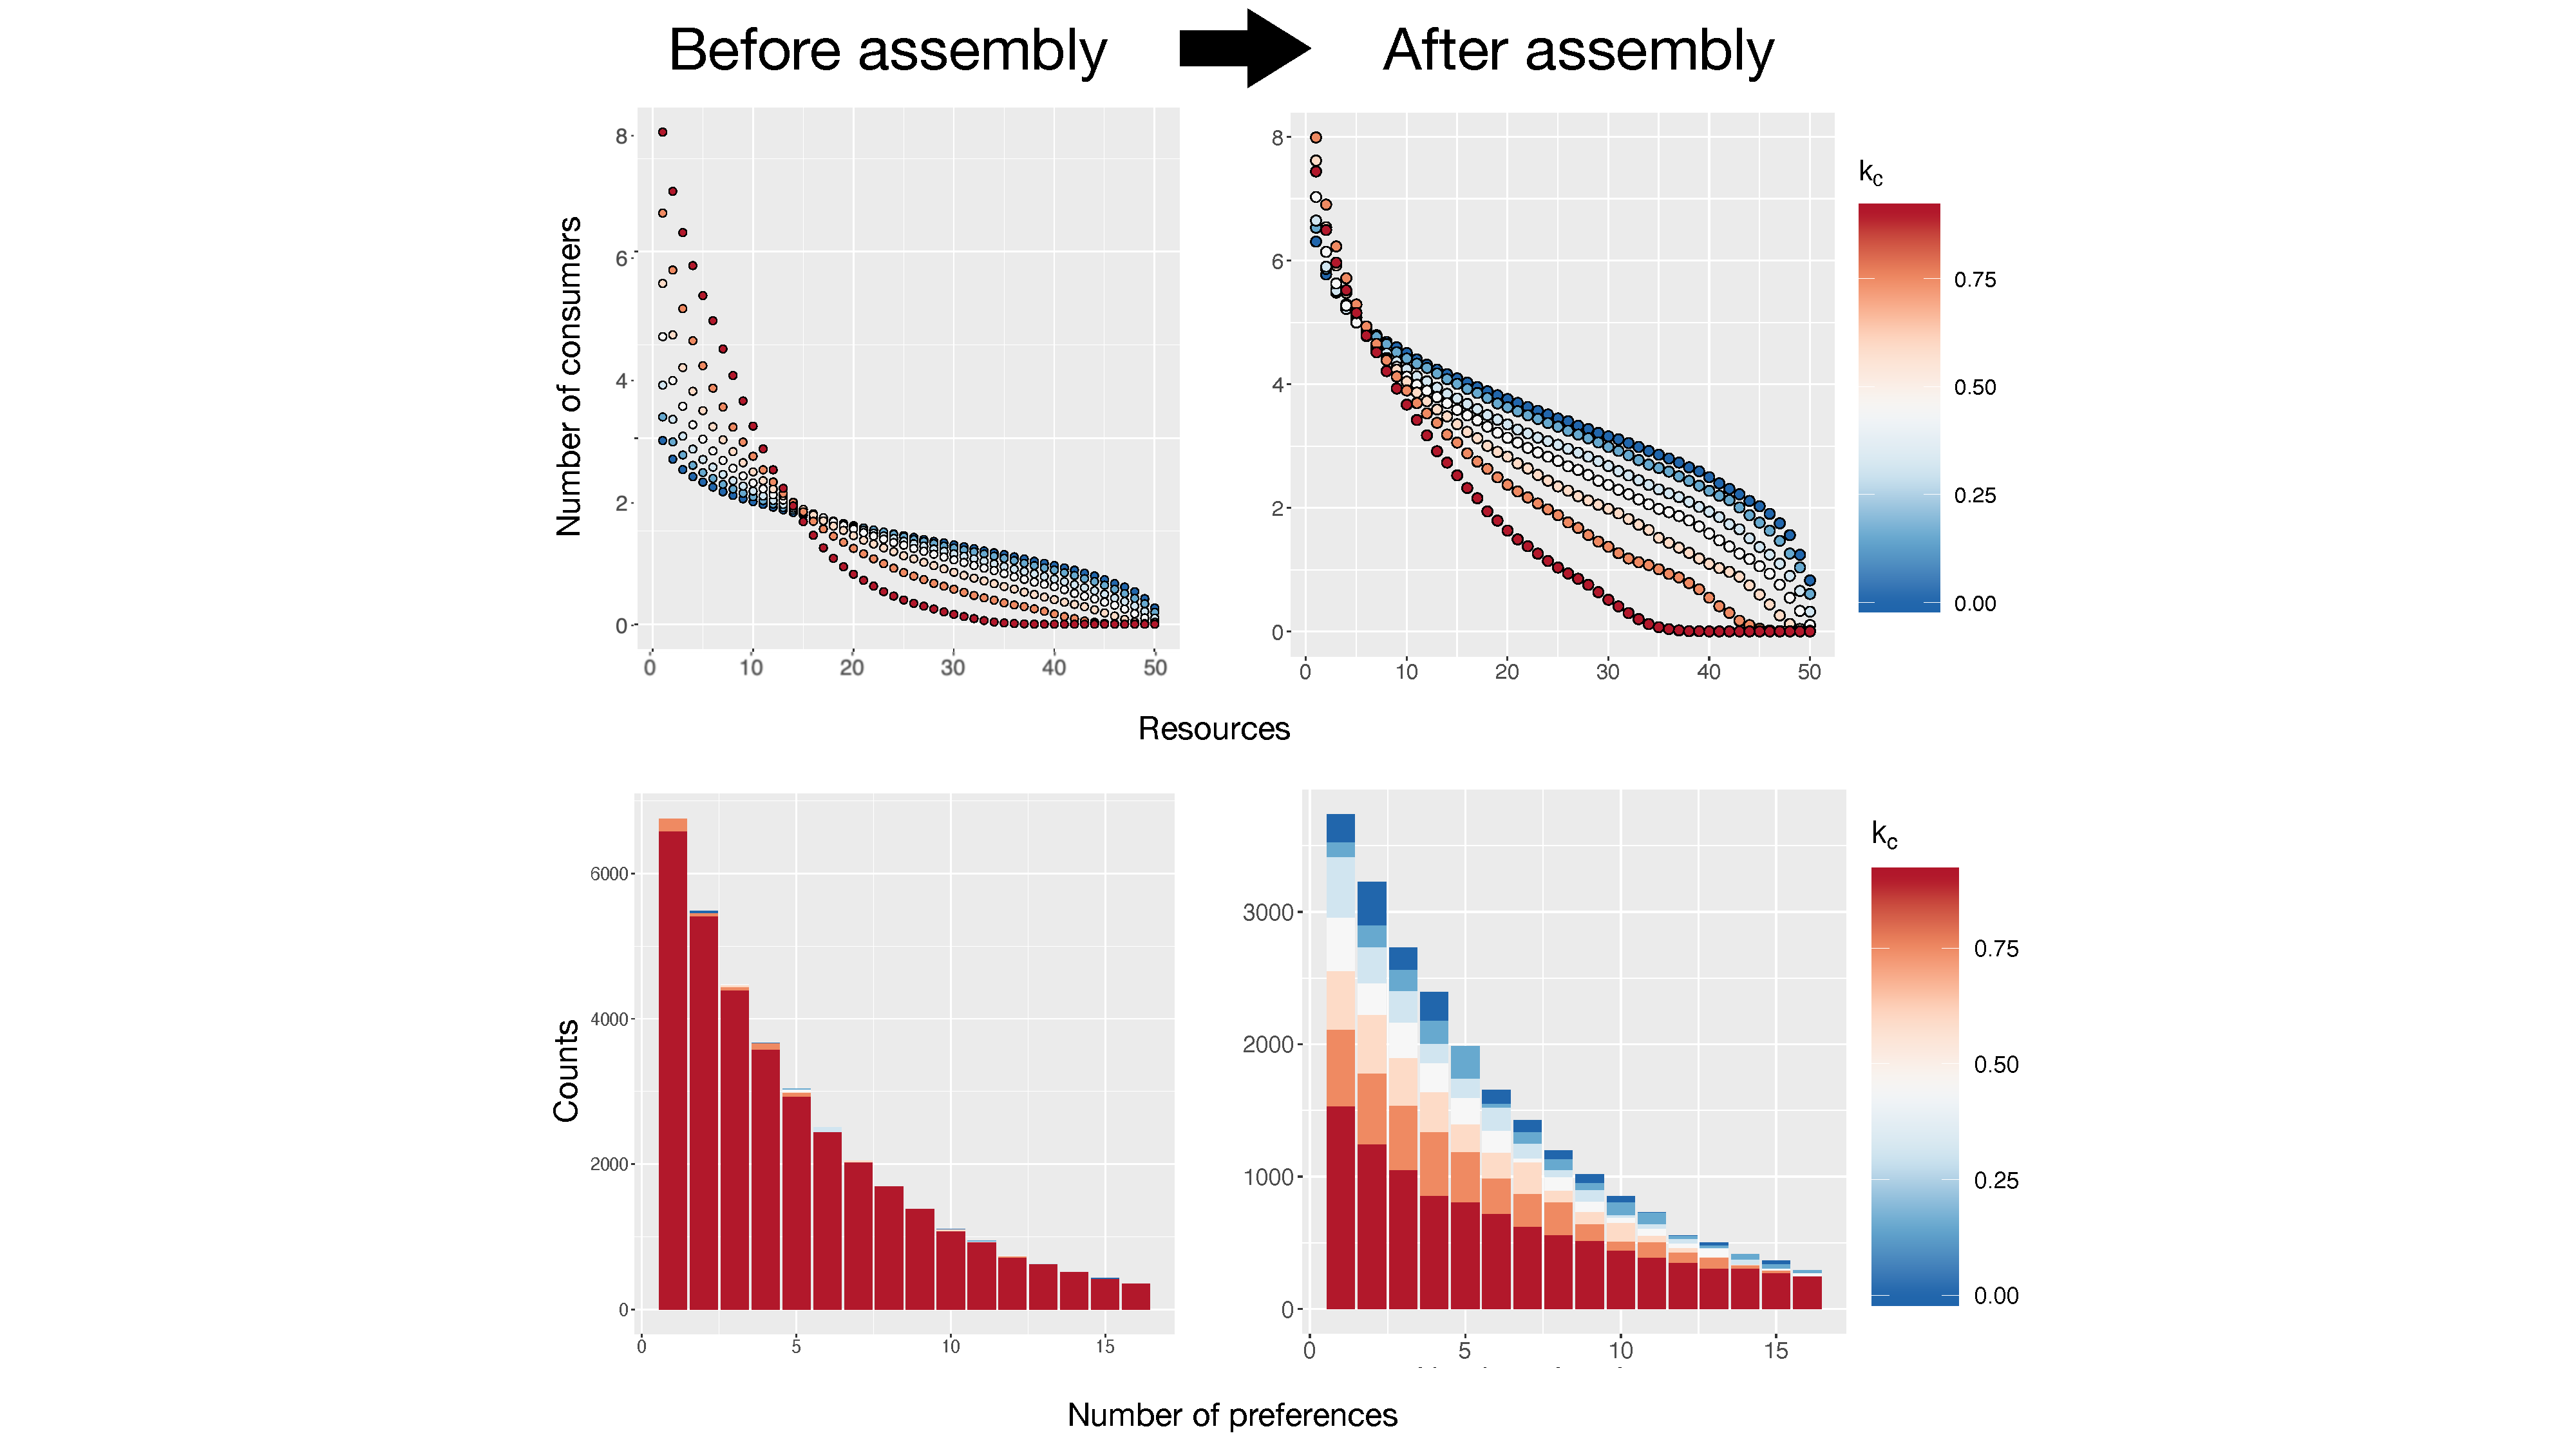
\includegraphics[width=0.9\textwidth]{before_after_assembly.pdf}
	\caption{\textbf{Top row}: number of consumers per resource (arbitrarily labelled before and after community assembly, for increasing value of the competitiveness factor. Note that as $k_c$ increases, the difference between the most demanded resource and the second-most demanded resource increases, for both the before, and after assembly cases. \textbf{Bottom row}: Histogram of number of consumers (y-axis) with $n_c$ (x-axis) number of preferences. We find that the trend does not change before and after assembly, since in both plots it the probability to posses $n_c$ preferences decreases as $n_c$ increases to have a higher amount of resource preferences.}
	\label{fig:before_after_assembly}
\end{figure}

We perform two sets of community assembly simulations. First, under preferential feeding, and second with resource guild structure added. Within each set, we perform 100 random assembly processes at every point of the parameter grid, which encompasses all possible combinations of the following parameter values $s = m = 60$, $l = k_c = k_f = [0.1,...,0.9]$. $K_c = K_f = 0$, in the first set, and $\in [0.1,...,0.9]$ in the second one. We then use the assembled communities to perform \textit{in silico} community invasion assays.

We also need to ensure that these non-random structures remain in place after the communities have been assembled. To this end, we plot the number of consumers per resource, before and after assembly, as a function of $k_c$, and also the histograms of the number of metabolic preferences before and after assembly for each value of $k_c$. As can be seen in Fig  \ref{fig:before_after_assembly}, the constraints on resource preferences, although slightly modified, remains in place. The difference in the number of consumers per resource is much higher for high $k_c$ than it is for lower values of $k_c$, corresponding with what we imposed before assembly. Likewise, the exponential distribution that we imposed on the number of preferences per consumer is also maintained after assembly, with slight differences in the final overall species richness values.

\begin{figure}[t]
	\centering
	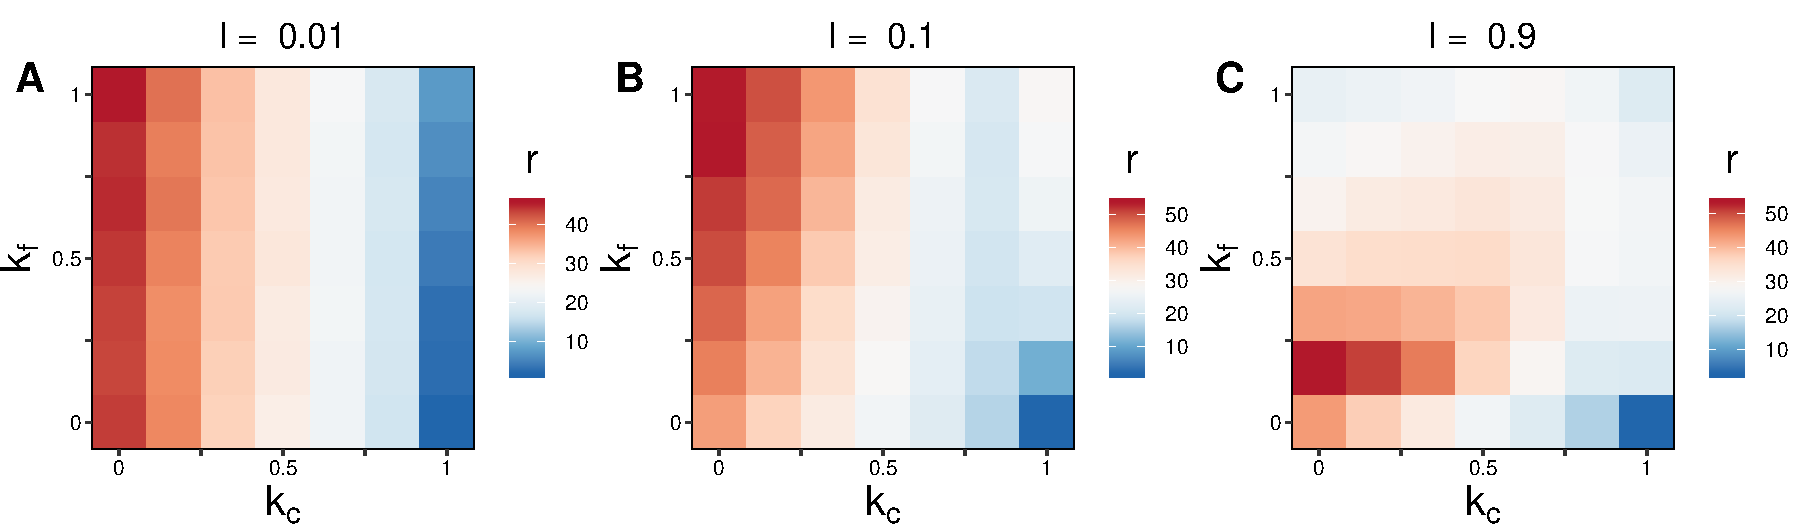
\includegraphics[width=\textwidth]{kc_kf_richness.pdf}
	\caption{Heat-maps for each value of $ l $ of the average richness $ r $ as a function of $ k_c $ and $ k_f $. {\bf A}: When leakage is negligible, average species richness decreases as $ k_c $ increases, but does not change with $ k_f $. That is, leakage is so low that the effect of the level of facilitation on the the final community richness is negligible.  {\bf B}: At intermediate leakage level, the average richness is maximized  where competition is lowest and facilitation highest, and  minimized under the exact opposite set of conditions. {\bf C}: At very high level of leakage, highest richness is reached in communities with low competition and facilitation levels.} 
	\label{fig:kc_kf_richness}
\end{figure}

Interestingly, after assembling the parent communities, we find that each value of leakage represents a different regime, resulting in different effects on species richness. The result in Fig \ref{fig:kc_kf_richness}C may seem particularly counter-intuitive, as one would expect that high facilitation promotes species diversity. However, the species in  this communities are not efficient at consuming resources, since they leak the majority of what they harvest. Thus, in order to most efficiently deplete the most efficiently  available resources, they need to perform more cycles of consumption than a species with a lower leakage factor. The optimal interaction topology that ensures efficient resource depletion in several cycles of consumption and leakage is one that minimizes facilitation and competition.   
To sum up; predictably, the three figures show that biodiversity is favoured by niche separation, since less competitive communities are more diverse. Surprisingly, the benefit of cooperative interactions changes for each case. For individuals in very low leakage communities, cooperative interactions are irrelevant. These become beneficial as leakage levels become moderate. However, they are detrimental, and therefore minimized in situations where leakage is high.

\section{Matrix representation of the model }\label{matrix_representations}

Here we describe the matrix form of the model system (Eq \ref{eq:model}), useful for efficient (vectorized) simulations. Eqs~\ref{eq:model} can be expressed in matrix form as:
\begin{equation*}
	\begin{aligned}
	\frac{d\boldsymbol{n}}{dt} &= \boldsymbol{g}\circ \boldsymbol{n}\left(D(\boldsymbol{R})C(\boldsymbol{1}-\boldsymbol{l}) - \boldsymbol{z}\right)\\
	\frac{d\boldsymbol{R}}{dt} &= \boldsymbol{\kappa} - D(\boldsymbol{R})C^T\boldsymbol{n} + D^TD(\boldsymbol{l}\circ \boldsymbol{R})C^T\boldsymbol{n}.
	\end{aligned}
\end{equation*}
Here, $\boldsymbol{1}$ is a column vector of ones of appropriate dimension, and $ \circ $ denotes an element-wise operation.
The interaction metrics  presented above can also be vectorized. In the following we use that the factor $\tilde{\kappa}_j = 1$ because in our simulations, all the resources are being supplied in the same amount. For instance, in the equations of competition, since metabolic preferences are binary, taking the scalar product of the two preference vectors yields the number of common elements between them.
\begin{equation*}
    	C_a = (1-l) CC^T
\end{equation*}
For Eq \ref{eq:biotic}, only indices $j$ and $k$ can be vectorized, taking the form
\begin{equation*}
    (C_b)_{\alpha \beta} = l \left(\vec{c_{\alpha}} + \vec{c_{\beta}}\right)^T D \left(\vec{c_{\alpha}}\circ \vec{c_{\beta}}\right)
\end{equation*}
The vectorization of Eq \ref{eq:facilitation} is expressed as
\begin{equation*}
    F = l C D C^T
\end{equation*}

\subsection*{Matrix representation at coalescence event}
Each coalescence event is simulated by mixing the species from each community after the assembly process in isolation has been completed. This can be mathematically expressed in matrix form through a system of $ s_1 + s_2 + m $ differential equations, where $ s_1 $ and $ s_2 $ are the number of species that remain in the first and second communities after their assembly, respectively: 
\begin{align}
	\frac{d\boldsymbol{n}_e}{dt} &= \boldsymbol{g}\circ \boldsymbol{n}_{e}\left(D(\boldsymbol{R}_e)C_{e}(\boldsymbol{1}-\boldsymbol{l}_e) - \boldsymbol{m}_e\right) \label{eq:extended_system_pop} \\ 
	\frac{d\boldsymbol{R}}{dt} &= \boldsymbol{\kappa} - \left[\mathbb{1} \ \mathbb{1}\right] \Big( D(\boldsymbol{R}_e)C_e^T\boldsymbol{n_e} +  D_e^TD(\boldsymbol{l_e}\circ \boldsymbol{R_e})C_e^T\boldsymbol{n}_e\Big) \label{eq:extended_system_rec}
\end{align}
Here $ \left[\mathbb{1} \ \mathbb{1}\right] $ represents the horizontal concatenation of two $m \times m$ identity matrices. The sub-index $e$ stands for \textit{extended}. To form any of the extended vectors in equations \ref{eq:extended_system_pop} and \ref{eq:extended_system_rec}, one simply vertically concatenates the vectors from community 1 and community 2. Constructing an extended matrix in Eq \ref{eq:extended_system_pop} and \ref{eq:extended_system_rec} is done by joining the two matrices alongside their diagonal. For example, constructing the vector of species abundances $\boldsymbol{n}_e$ and the metabolic matrix $D_e$ would be done as
\begin{equation*}
    \boldsymbol{n}_e = \begin{bmatrix}
                            \boldsymbol{n}^{(1)} \\
                            \boldsymbol{n}^{(2)} \\
                        \end{bmatrix} 
    \qquad \qquad \qquad 
    D_e = \begin{bmatrix}
                D^{(1)} & 0 \\
                0 & D^{(2)} \\ 
          \end{bmatrix},
\end{equation*}
where the superscripts indicate membership of community (1 or 2).

%\section{Table of parameter values}\label{parameter_values}

%Table of parameter values!

\newpage

\bibliographystyle{agsm}
\bibliography{references}

\end{document}